\clearpage
\sect{5. The story}
Mad Mix has restored peace to Cocovillage, but his cousin Ope faces a new nightmare in Cococastle. A surviving coco has taken refuge in the castle and joined its sinister inhabitants. Mad must come to the rescue once more.


\sect{6. How to play}
Explore the corridors and collect cocos to progress through the castle. Avoid enemies and traps; use your jump to overcome obstacles.

There are nine stages. Completing the ninth returns you to the first. Each stage is announced before play begins. If you lose a life, you return to the stage's starting position; cocos already collected remain collected.

Mad stays centred while the scenery scrolls around him; jumping retains its vertical movement. Movement and animation keep a regular cadence; music retains its normal tempo.

\textbf{STANDARD} keeps regular movement speed. \textbf{HARD} doubles base movement for Mad and other actors. Mad\textquotesingle{}s speed boost has the same maximum in both modes.

\sect{7. The screen}
\begin{center}
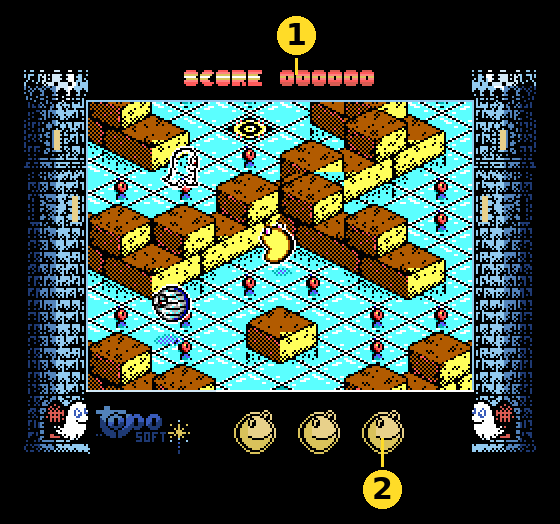
\includegraphics[width=0.68\textwidth]{img/hud.png}
\end{center}
\begin{tabularx}{\textwidth}{@{}clX@{}}
\toprule No. & Element & Meaning\\\midrule
1 & \texttt{SCORE} & Points accumulated during the current game.\\
2 & Yellow faces & Reserve lives; the life currently in use is not shown.\\
\bottomrule
\end{tabularx}

\clearpage
\sect{8. Points, lives and tips}
You start with one active life and three reserves. An empty life display still leaves you with the life in play. Extra lives can raise your reserves to four.

A normal coco adds one point, except when it triggers a collection bonus. Other pickups and effects can award different amounts. \texttt{SCORE} resets when you begin a new game.

\begin{itemize}
\item Hold \key{F1} while dismissing the opening illustration with Space or fire to avoid contact damage from ghosts, Dracula and Franky. Balls and traps remain dangerous.
\item Press and release fire for each jump; holding it does not chain jumps.
\item Push corks into enemy exits to block them temporarily. Catch the fleeing accelerator again to gain its speed boost.
\item Push balls toward monsters and keep clear of their path once they roll.
\item Use \key{H} when you need a break. \key{V} silences the music.
\end{itemize}
